% UTF-8

% single-chapter commands
\documentclass[../main/thesis.tex]{subfiles}
\onlyinsubfile{\setcounter{chapter}{3}}  % single-chapter command
\begin{document}


\chapter{Algorithmen zur Generalisierung}

\section{Vorüberlegungen}

% Erst über Generalisierung nachgedacht, da sie das schwierigerer Problem zu sein schien (in der Erwartung, die Identifikation ließe sich evtl. "nebenbei" lösen).
% Die Generalisierung ist auf den allerersten Blick ein einfaches geometrisches Problem, das keiner ausgefeilten Algorithmen a la 2.5 bedarf. Erst mal probiert, ob es sich so lösen lässt. Später festgestellt (-> Implementierung?), dass es in der Tat nicht so schrecklich schwierig war, jedoch die Entscheidung, was zusammengehört und was nicht, im Allgemeinen Fall schwieriger als erwartet war (ein Problem, das allerdings wohl auch für die Lösungen aus 2.5 bestanden hätte, womöglich gar in verstärktem Ausmaß).

% an dieser Stelle außerdem __Überleitung__: was kann man aus 2.5 für lehren/erkenntnisse ziehen? irgendwas anwendbares dabei? wenn ja, warum nicht?

Aus der Menge der zuvor erwähnten bereits existierenden Ansätze hebt sich zunächst die Skelettierung heraus, weil es für sie bereits mehrere funktionale Implementierungen der Zusammenfassung gibt (Abschnitt~\ref{ch:skeleton}).
Diese haben jedoch laut der Autoren alle mit erheblichen Problemen in Kreuzungsbereichen zu kämpfen, die nur teilweise automatisiert gelöst werden können.
Dieser Ansatz erscheint wenig vielversprechend.

Letzteres gilt auch für den in Abschnitt~\ref{ch:conflict-detection} diskutierten Ansatz zur Konflikterkennung.
Zwar wäre eine Kombination mit anderen Ansätzen denkbar.
So könnte möglicherweise eine Pufferung der Linienzüge mit anschließender Verschneidung der entstehenden Flächen Informationen über die Linienzüge liefern:
Dort, wo sich Schnittflächen bilden, bestehen Konflikte;
Konflikte zwischen zwei Linien über große Teile ihrer Länge hinweg wären ein Indiz für Parallelität.
Dies löst jedoch nicht das Problem der Zusammenfassung beider Linien (vgl. Abschnitte~\ref{ch:buffer} und~\ref{ch:skeleton}).

Interessanter erscheint der bereits in Abschnitt~\ref{ch:graph-based} erwähnte Gedanke, dass Straßen mit parallelen Richtungsfahrbahnen oft komplex modellierte Kreuzungen haben.
Können diese zu jeweils einzelnen Knoten generalisiert werden, dann sind die parallelen Richtungsfahrbahnen im Graphen des Straßennetzes zwei gegenläufige gerichtete Kanten.
Anschließend wäre die geometrische Zusammenfassung dieser Kanten möglicherweise einfach.

% "perceptual grouping": nicht vielversprechend

Der von \citeauthor{Tho05} beschriebene Ansatz zur Generalisierung der OS~MasterMap klingt vielversprechend (Abschnitt~\ref{os-mastermap}).
Er kombiniert Ideen aus der visuellen Wahrnehmung \term{(strokes)} und der Graphenanalyse, um Richtungsfahrbahnen zusammenzufassen.
Den Erfolg seiner Methode schreibt er jedoch unter anderem der gründlichen Klassifikation seiner Ausgangsdaten nach Bauart der Straße zu (einbahnig/zweibahnig usw.). \cf[14]{Tho05}
Diese existiert in dieser Form nicht in OpenStreetMap, so dass seine Methode nicht direkt übertragbar erscheint.

Zwar kann für Autobahnen davon ausgegangen werden, dass sie zweibahnig ausgebaut sind.
Seltene Ausnahmen wie etwa die Bundesautobahn~62 zwischen Landstuhl und Pirmasens sollten, wenn sie denn tatsächlich als \osmtag{highway}[motorway] eingetragen sind, das Attribut \osmtag{oneway}[no] tragen und sich so identifizieren lassen.
Im übrigen Straßennetz sind solche Aussagen auf Basis der \osm-Daten jedoch nicht möglich.

Es ist ohnehin fraglich, wie stark die von \citeauthor{Tho05} eingesetzte Erkennung von \term{strokes} als möglichst \emph{lange} Linienzüge die Generalisierung im Kontext von \osm\ tatsächlich vereinfachen würde.
Zwar sind die einzelnen \term{ways} in \osm\ wegen ihrer ungleichmäßigen Aufteilung oft nicht gut zur Weiterverarbeitung geeignet.
Allerdings wären zur Prüfung auf Parallelität und zur Zusammenfassung auf eine gemeinsame Mittellinie auch möglichst \emph{kurze} Linienfragmente gut geeignet, sofern die Fragmentierung beider Parallelen gleichmäßig ist.

Im folgenden Abschnitt~\ref{ch:algorithm-principle} wird in allgemeinen Begriffen beschrieben, wie parallele Linienzüge auf Basis einer solchen gleichmäßigen Fragmentierung zusammengefasst werden können.
Im Anschluss daran folgt die formale Beschreibung dieser Algorithmen.

% erst Grundprinzip / -idee / -ansatz beschreiben, dann Edge Cases



\section{Grundprinzip}
\label{ch:algorithm-principle}

Um das Zusammenfassen paralleler Linienzüge vorzubereiten, werden alle \term{nodes} des einen Linienzugs jeweils einem gegenüberliegenden \term{node} auf dem parallelen Linienzug zugeordnet.
Die Verbindung der Mittelpunkte zwischen den so einander zugeordneten \term{nodes} ergibt direkt den zusammengefassten Linienzug als Ergebnis der Generalisierung (Abbildung~\ref{fig:general-approach}).

Dieses Vorgehen vermeidet, dass die in Abschnitt~\ref{ch:osm-intro} besprochene häufige ungleichmäßige Fragmentierung von \osm-Linienzügen in mehrere \term{ways} einen Einfluss auf den Generalisierungsvorgang hat.
Aufgrund der nicht immer gleichen Anzahl und Verteilung der \term{nodes} kommt es vor, dass ein \term{node} des einen Linienzugs mehreren \term{nodes} des anderen Linienzugs zugeordnet wird, was jedoch unproblematisch ist.

\twofigures{ht}{
	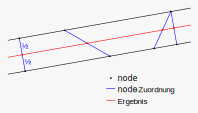
\includegraphics[width=\ScaleIfNeeded]{../chapter4/general-approach}
	\caption{Linienzusammenfassung durch Mittelpunktbildung nach Zuordnung gegenüberliegender \term{nodes}}
	\label{fig:general-approach}
}{
	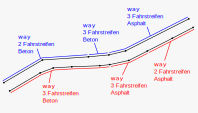
\includegraphics[width=\ScaleIfNeeded]{../chapter4/motorway-fragments}
	\caption{ungleichmäßige Fragmentierung paralleler Linienzüge (Beispiel)}
	\label{fig:motorway-fragments}
}

Um zwei gegenüberliegende \term{nodes} einander zuordnen zu können, müssen zunächst die Linien, deren Teil sie sind, als zueinander parallel erkannt werden.
Auch hierbei ist die erwähnte ungleichmäßige Fragmentierung in bestimmten Fällen problematisch.
Beispielsweise müssten die einzelnen \term{ways} in Abbildung~\ref{fig:motorway-fragments}, aus denen die beiden dargestellten Parallelen bestehen, zunächst zu einem längeren Linienzug verknüpft werden, um einen Vergleich zu ermöglichen.
Dies entspräche dem in Abschnitt~\ref{os-mastermap} beschriebenen Ansatz von Thom, der damit zufriedenstellende Resultate erzielte, dabei jedoch die hohe Qualität seiner Ausgangsdaten betonte, welche bei wie für \osm\ von Freiwilligen erfassten Geodaten nicht vorausgesetzt werden kann.

Um diese Problematik zu umgehen, verwendet das in dieser Arbeit vorgestellte Verfahren möglichst \emph{kurze} Liniensegmente anstelle möglichst \emph{langer} Linienzüge.
Die Verbindung zweier benachbarter \term{nodes} in einem \term{way} als kürzestmögliche lineare Einheit in den \osm-Ausgangsdaten (früher als \term{segment} bezeichnet \cf[57]{RT09}) ist allerdings für einen Vergleich nicht viel besser geeignet als der vollständige \term{way}%
% warum nicht? (wenig spezifisch formuliert)
, wie aus Abbildung~\ref{fig:motorway-fragments} ersichtlich ist.
% nicht wirklich gut ersichtlich; neue Abbildung mit Pfeilen wie in fig:comparable-fragments?
Daher werden die \term{segments} vor der Analyse auf Parallelität solange immer weiter unterteilt, bis schließlich ein einfacher geometrischer Vergleich möglich ist (Abbildung~\ref{fig:comparable-fragments}).

\onefigure{ht}{
	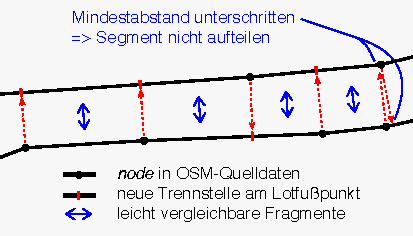
\includegraphics[width=\ScaleIfNeeded]{../chapter4/comparable-fragments}
	\caption{Herstellung einer gleichmäßigen Fragmentierung paralleler Linienzüge}
	\label{fig:comparable-fragments}
}



\section{Operationen}
\label{ch:algorithm-parts}

Der zuvor beschriebene Lösungsansatz lässt sich vereinfacht als Sequenz von vier Operationen ausdrücken:
\begin{enumerate}[nosep]
	\item Segmente unterteilen
	\item Analysieren
	\item Punktezuordnung
	\item Parallelen zusammenfassen
\end{enumerate}
%
Die folgenden Abschnitte beschreiben jede dieser Operationen im Detail.
Verwendete mathematische Symbole werden in Anhang~\ref{appx:mathsymbols} erklärt.



\subsection{Segmente unterteilen}
\label{ch:split-algorithm}

In \osm-Daten sind seit Oktober~2007 Segmente (Verbindungen von exakt zwei \term{nodes}) nicht mehr als eigene Objekte enthalten \cf[57]{RT09}.
Anhand der aus der Datenquelle eingelesenen Menge aller \term{ways} wird daher zunächst die Menge aller \textproc{Segmente} ermittelt (Abbildung~\ref{fig:segments-in-way}).

\onefigure{ht}{
	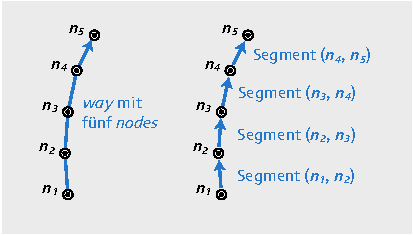
\includegraphics[width=\ScaleIfNeeded]{../chapter4/segments-in-way}
	\caption{vier Segmente in einem \term{way} (Beispiel)}
	\label{fig:segments-in-way}
}
\onefigure{!ht}{
	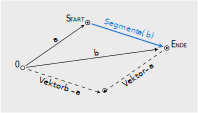
\includegraphics[width=\ScaleIfNeeded]{../chapter4/vector-geometry}
	\caption{einfache Vektorgeometrie an einem Segment demonstriert}
	\label{fig:vector-geometry}
}

Um Verbindungen zwischen zwei \term{nodes} deterministisch beschreiben zu können, werden diese hier als Kanten in einem gerichteten Graphen betrachtet.
Die beiden \term{nodes} werden im Folgenden als \textproc{Start} und \textproc{Ende} bezeichnet; es gilt:
% evtl. besser \textproc{Ziel}, um Oberbegriff "Endpunkt" freizuhalten
\[
\Set{\textproc{Start}(s), \textproc{Ende}(s)} = \textproc{Nodes}(s)\ \forall\ s
\]

Geometrisch betrachtet entsprechen \term{nodes} Punkten, die durch vom Koordinatenursprung ausgehende Vektoren in der euklidischen Ebene definiert sind.
Segmente als gerichtete Verbindungen zweier solcher Punkte lassen sich dann ebenfalls als Vektoren auffassen und als geordnetes Paar notieren.

So könnten beispielsweise die Ortsvektoren $a$ und $b$ das Segment $(a,b)$ definieren, welches geometrisch zum freien Vektor $b - a$ kongruent wäre (Abbildung~\ref{fig:vector-geometry}).

\begin{algorithmhere}{Segmentierung}
\label{alg:Segmentierung}
\begin{algorithmic}
\Function{Segmente}{$W$}\Comment{Menge aller \term{ways} $W$}
	\State \textbf{Ergebnis} sei die Menge aller Segmente $(n, n')$ für Paare von Punkten jedes Linienzugs $w \in W$ derart, dass $n$ Vorgänger von $n'$ im Verlauf von $w$ ist.
\EndFunction
\end{algorithmic}
\end{algorithmhere}
% implementiert in OsmWay.segmentation()

% "anschließend" ergibt einen etwas holprigen Übergang

Die Segmente werden anschließend durch \textproc{Splitten} derart aufgeteilt, dass ein geometrischer Vergleich leicht möglich wird (Abbildung~\ref{fig:comparable-fragments}).
Die so entstehenden Fragmente sind keine Segmente im Sinne der früheren gleichnamigen \osm-Objekte, da der Punkt, an dem sie zerteilt wurden, keinen \term{node} in OpenStreetMap darstellt.
Im Folgenden werden sie dennoch vereinfachend Segmenten gleichgestellt, da sie ansonsten dieselben Eigenschaften besitzen.

Aufgeteilt werden Segmente jeweils am \textproc{Fußpunkt} eines Lots, das von einem \term{node} eines anderen Segments gefällt wird.
Der gewählte Algorithmus für das \textproc{Splitten} arbeitet geometrisch rekursiv:
Alle erzeugten Fragmente werden wieder zur Menge der Segmente hinzugefügt und somit immer weiter aufgeteilt, bis kein \textproc{Fußpunkt} mehr gefunden wird.

% TODO: Grafik (unbedingt!), um "rekursiv" zu illustrieren

\begin{algorithmhere}{Splitten}
\label{alg:Splitten}
\begin{algorithmic}
\State $\textbf{Relation}\ \relation{wurzel} : \textrm{Segment} \rightarrow \textrm{Segment}$
\State $\textbf{Anfangswert}\ \relation{wurzel}[s] \eqdefrel s\;\forall\ s$
\Function{Splitten}{$S$}\Comment{Menge aller Segmente $S$}
	\State $S' \gets S$
	\ForAll{$s \textbf{ mit } s \in S'$}
		\ForAll{$n \textbf{ mit } n \in \Set{\textproc{Start}(s), \textproc{Ende}(s)} $}
			\State $T \gets \textproc{NaheSegmente}(s, S')$
			\ForAll{$t \textbf{ mit } t \in T \wedge \exists\ f : f = \textproc{Fußpunkt}(n, t)$}
				\State $t_1 \gets (\textproc{Start}(t), f)$
				\State $t_2 \gets (f, \textproc{Ende}(t))$
				\State $S' \gets \Set{t_1, t_2} \cup S' \setminus \Set{t}$\Comment{$t$ ersetzen durch Fragmente $t_1$ und $t_2$}
				\State $\relation{wurzel}[t_1] \gets \relation{wurzel}[t]$
				\State $\relation{wurzel}[t_2] \gets \relation{wurzel}[t]$
			\EndFor
		\EndFor
	\EndFor
	\State \textbf{Ergebnis} $S'$
\EndFunction
\end{algorithmic}
\end{algorithmhere}
% implementiert in Combiner.splitSegments()

Es ist nicht notwendig, jedes Segment mit allen anderen Segmenten zu vergleichen.
Segmente, die zu weit entfernt und somit nicht \textproc{NaheSegmente} sind, können von vornherein als potenzielle Parallelen ausgeschlossen werden.
Zur Entscheidung, welche Segmente als „nah“ gelten und damit für Parallelität in Frage kommen, wird für jedes Segment eine \textproc{Hülle} gebildet, welche etwas größer als das jeweilige Segment ist, so dass sich die Hüllen von nahe beieinander liegenden Segmenten überschneiden.
% TODO: Grafik und/oder Literaturverweis

\begin{algorithmhere}{nahe Segmente}
\label{alg:NaheSegmente}
\begin{algorithmic}
\Function{NaheSegmente}{$s, S$}\Comment{Menge aller Segmente $S$}
	\State \textbf{Ergebnis} $\Set{t \in S \SetCond \textproc{Hülle}(s) \cap \textproc{Hülle}(t) \neq \Nil}$
\EndFunction
\end{algorithmic}
\end{algorithmhere}
% implementiert in Combiner.regionaliseSegments()
% abweichend wird dort das Ergebnis für alle s berechnet und gecached

% TODO: Diese Definition weicht vereinfachend vom ursprünglichen Entwurf ab,
% indem alle nahen Segmente geliefert werden statt nur solche, die gleich
% ausgerichtet sind (closeSegments/closeParallels). Tests zeigen, dass diese
% Vereinfachung unzulässig ist: Das Ergebnis wird verschlechtert, weil so
% halt gerade an Kreuzungen und Querungen lauter Splits entstehen, die kein
% Mensch braucht, was die Analyse erschwert (und sicher auch ineffizient
% ist). NAHESEGMENTE muss entweder entsprechend korrigiert oder aber die
% Beschreibung entsprechend ergänzt werden. Außerdem liefert diese Definition
% fälschlich auch "s" selbst zurück, was sich allerdings durch ein einfaches
% "\wedge s \neq t" lösen lässt.

Als \textproc{Hülle} könnte ein Puffer dienen.
Aus Gründen der Effizienz bietet es sich jedoch an, die \textproc{Hülle} rechteckig im Koordinatennetz anzulegen.
Für diesen Fall hängt die Größe der Hülle auch von der Orientierung des Segments ab.
Im Ergebnis wird dann später zu sehen sein, dass diagonal zum Koordinatennetz ausgerichtete Segmente bei größeren Abständen zueinander als parallel erkannt werden als solche Segmente, die orthogonal zum Koordinatennetz ausgerichtet sind.

Um die Korrektheit der Algorithmen sicherzustellen, ist aus diesen Gründen in der späteren \textproc{Analyse} auf Parallelität eine erneute Prüfung des tatsächlichen Abstands zweier zu vergleichender Segmente notwendig.
Diese kann dann jedoch auf \textproc{NaheSegmente} beschränkt werden und ist dementsprechend billig (vergleiche Abschnitt~\ref{ch:analyse-algorithm}).

Weiterhin hängen diese Erkennungsabstände vom gewählten Koordinatennetz ab.
Würde beispielsweise mit geographischen Koordinaten gearbeitet, so variiert das Verhältnis der Erkennungsabstände in Ost/West- und in Nord/Süd-Richtung mit der geographischen Breite.
Für geometrische Operationen in der euklidischen Ebene bieten sich jedoch nur winkeltreue Abbildungen mit geringen Maßstabsfehlern im Anwendungsgebiet an. \cf[20]{Sny87}

% TODO: Grafik?

\begin{algorithmhere}{Definition der erweiterten Hüllfunktion für \textproc{NaheSegmente}}
\label{alg:Huelle}
\begin{algorithmic}
\Function{Hülle}{$s$}
	\State \textbf{Ergebnis} sei die nach allen Kardinalrichtungen um $\eta/2$ vergrößerte rechteckige Hülle um das Segment $s$, wobei $\eta$ der festzulegende Höchstabstand sei, für den zwei Segmente als „nahe“ gelten dürfen.
\EndFunction
\end{algorithmic}
\end{algorithmhere}
% implementiert in SourceSegment.envelope()

\noindent
Das Aufteilen in Fragmente erfolgt jeweils am \textproc{Fußpunkt}~(Abbildung~\ref{fig:footpoint}).

\begin{algorithmhere}{Fußpunkt}
\label{alg:Fusspunkt}
\begin{algorithmic}
\Function{Fußpunkt}{$n,t$}
	\State \textbf{Ergebnis} sei der Lotfußpunkt~$f$ des Punkts~$n$ auf der Geraden~$t$. Liegt~$f$ nicht zwischen den Punkten $\textproc{Start}(t)$ und $\textproc{Ende}(t)$ oder liegt~$f$ näher an $\textproc{Start}(t)$ oder $\textproc{Ende}(t)$ als die festzulegende Mindestlänge~$\mu$ eines Fragments, dann gibt es kein Ergebnis.
% Der zweite Satz ist ein wesentliches, aber nicht unbedingt offensichtliches Detail, deshalb sollte auch das an sich einfache Konzept "Lotfußpunkt" formal beschrieben werden.
\EndFunction
\end{algorithmic}
\end{algorithmhere}
% implementiert in AbstractSegment.findPerpendicularFoot()

\onedoublefigure{H}{
	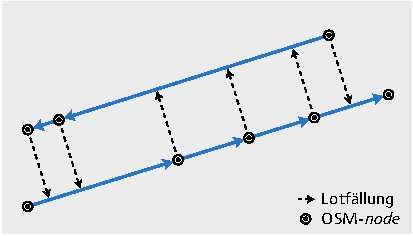
\includegraphics[width=\ScaleIfNeeded]{../chapter4/footpoints1}%
}{
	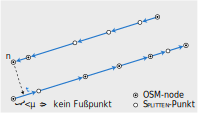
\includegraphics[width=\ScaleIfNeeded]{../chapter4/footpoints2}%
}{
	\caption
		[Bestimmung der Punkte, an denen Segmente aufzuteilen sind]
		{Bestimmung der Punkte, an denen Segmente aufzuteilen sind (links vor, rechts nach dem \textproc{Splitten})}
	\label{fig:footpoint}
}



\subsection{Analysieren}
\label{ch:analyse-algorithm}

Das Ergebnis der Operation „Segmente unterteilen“ eignet sich zur \textproc{Analyse} auf Parallelität.
Hierfür werden Geometrie und Attribute näher verglichen mit dem Ziel, für jedes Segment beidseitig entweder genau ein oder kein anderes Segment als „parallel“ zu kennzeichnen.
% (dies funktioniert, weil bei ungleichmäßiger Fragmentierung die Verknüpfung über das _andere_ Segment hergestellt wird, d. h. dies ergibt keine 1:1-Beziehung)
%
Die Unterscheidung der Seiten links und rechts kann durch Bestimmung der Winkel zu den \term{nodes} des jeweils anderen Segments erfolgen (Abbildung~\ref{fig:left-side}).

\onefigure{ht}{
	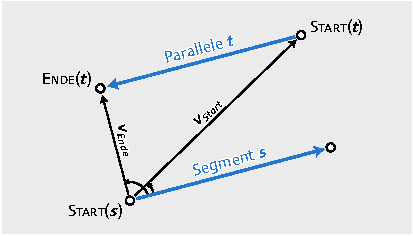
\includegraphics[width=\ScaleIfNeeded]{../chapter4/left-side}
	\caption{Erkennen einer nahen Parallele auf der linken Seite eines Segments}
	\label{fig:left-side}
}

\begin{algorithmhere}{Analyse}
\label{alg:Analyse}
\begin{algorithmic}
\State $\textbf{Relation}\ \relation{parallelLinks} : \textrm{Segment} \rightarrow \textrm{Segment}$
\State $\textbf{Anfangswert}\ \relation{parallelLinks}[s] \eqdefrel \Nil\ \forall\ s$
\State $\textbf{Relation}\ \relation{parallelRechts} : \textrm{Segment} \rightarrow \textrm{Segment}$
\State $\textbf{Anfangswert}\ \relation{parallelRechts}[s] \eqdefrel \Nil\ \forall\ s$
\Function{Analyse}{$S$}\Comment{Menge aller \emph{unterteilten} Segmente $S$}
	\ForAll{$s \textbf{ mit } s \in S$}
%		\State $T \gets \{t : wurzel(t) \in \textproc{NaheSegmente}(wurzel(s), S)\} \wedge \textproc{Parallel}(s, t)$  % exakt wie implementiert, aber eigentlich in dieser Form hier nicht nötig
		\State $T \gets \Set{t \SetCond t \in \textproc{NaheSegmente}(s, S) \wedge \textproc{Parallel}(s, t)}$  % vereinfachend
		\State $v_{Start} \gets \textproc{Start}(t) - \textproc{Start}(s)$
		\State $v_{Ende} \gets \textproc{Ende}(t) - \textproc{Start}(s)$
		\State $\mathtowidth[R]{L} \gets \Set{t \in T \SetCond \sphericalangle (s, v_{Start}) < 0 \wedge \sphericalangle (s, v_{Ende}) < 0}$
		\State $R \gets \Set{t \in T \SetCond \sphericalangle (s, v_{Start}) > 0 \wedge \sphericalangle (s, v_{Ende}) > 0}$
		\State\Comment{Mengen $L, R$ aller nahen Parallelen links- bzw. rechtsseitig}
		\State\Comment{Winkel seien definiert im Intervall $(-\pi,\pi)$ und im Uhrzeigersinn}
		\ForAll{$\mathtowidth[r]{l} \textbf{ mit } \mathtowidth[r]{l} \in L$}
			\If{$0 < \textproc{Distanz}(s, \mathtowidth[r]{l}) \leqslant \textproc{Distanz}(s, \mathtowidth[r']{l'})\; \forall\ \mathtowidth[r']{l'} \in L$}
				\State $\relation{parallelLinks}[\relation{wurzel}[s]] \gets l$
			\EndIf
		\EndFor
		\ForAll{$r \textbf{ mit } r \in R$}
			\If{$0 < \textproc{Distanz}(s, r) \leqslant \textproc{Distanz}(s, r')\; \forall\ r' \in R$}
				\State $\relation{parallelRechts}[\relation{wurzel}[s]] \gets r$
			\EndIf
		\EndFor
	\EndFor
	\State \textbf{Ergebnis} $\relation{parallelLinks}, \relation{parallelRechts}$
\EndFunction
\end{algorithmic}
\end{algorithmhere}
% implementiert in AbstractSegment.analyse()

% Die hier gewählte Definition findet für jede Seite jedes Segments höchstens ein PARALLELes Segment. Alternative wäre auch eine Definition möglich, die *jedes* PARALLELe Segment findet, weil beim NODESZUORDNEN durch die Mengeneigenschaften die Richtung der Zuordnung keine Rolle spielt und Duplikate ignoriert werden. Die Frage ist im Kern, was leichter zu verstehen ist ("parallelLinks" wäre dann eine Relation auf eine Menge von Segmenten, dafür entfiele die Prüfung ∀l' / ∀r').
% Welche Variante auch immer gewählt wird: Auf die Wahlfreiheit sollte irgendwo in 4.3 hingewiesen werden (derzeit hier weiter unten, als Fußnote). Dies wurde auch experimentell überprüft (CorrelationGraph-realParallels-reciprocity-check).

% reicht es evtl. aus festzulegen: 2 Segmente parallel gdw. mind. je ein Fragment parallel ist? dann wäre es danach nur noch eine frage, das "beste" zu finden
% oder evtl. statt "<- l" einfach "<- wurzel(l)" und dann das als Menge ausführen? Das könnte der tatsächlichen Implementierung am ehesten entsprechen, ist aber evtl. unnötig kompliziert.

Dabei kommen nur solche Segmente für die Kennzeichnung in Frage, die im Kontext des jeweiligen Anwendungsfalls als \textproc{Parallel} gelten (vergleiche Kapitel~3).

\begin{algorithmhere}{Parallel}
\label{alg:Parallel}
\begin{algorithmic}
\Function{Parallel}{$s_1, s_2$}
	\State Die Segmente $s_1$ und $s_2$ seien parallel genau dann, wenn sie:
	\begin{itemize}[nosep,leftmargin=3.5em]
		% [SourceSegment.closeParallels]
		\item ähnlich ausgerichtet sind (z.~B. $\alpha \eqdef \abs\sphericalangle (s_1, s_2)\abs < 15\degree$),
		% [MyAnalyser.shouldEvaluate]
		\item nahe beieinander liegen (z.~B. $\eta \eqdef \textproc{Distanz}(s_1, s_2) < \unit[40]{m}$),
		\item nicht so sehr zueinander versetzt sind, dass sie mehr hintereinander als nebeneinander liegen,  % "ignore collinear fragments"; sollte durch die geschickte Fragmentierung normal nicht vorkommen
		\item sich nicht überkreuzen,  % (sollte bereits durch \textproc{Analyse} ausgeschlossen sein)
		\item Teile von \term{ways} mit dem gleichen Wert für \osmtag{highway}[*] sind und
		\item Teile von \term{ways} mit dem gleichen Wert für \osmtag{ref}[*] sind.
	\end{itemize}
\EndFunction
\end{algorithmic}
\end{algorithmhere}
% implementiert in SourceSegment.closeParallels() und MyAnalyser

% Distanz 40 m:
% - vgl. https://de.wikipedia.org/wiki/Richtlinien_f%C3%BCr_die_Anlage_von_Autobahnen
% - Regelquerschnitt einer breiten Autobahn beträgt etwa 36 bis 44 m
% - theoretisch ist die Distanz die Hälfte des RQ, jedoch wird etwas Puffer benötigt, weil die Linienzüge in OSM meist nicht optimal gezeichnet sind und zudem stellenweise die Autobahnen etwas breiter als üblich gebaut sind

Dass die miteinander verglichenen Segmente nahe beieinander liegen, wird in der \textproc{Analyse} bereits durch die Beschränkung auf \textproc{NaheSegmente} sichergestellt.
Welche Segmente als „nah“ gelten, ist jedoch von der Definition der \textproc{Hülle} abhängig, für die Überlegungen zur Effizienz eine Rolle spielen (vergleiche Abschnitt~\ref{ch:split-algorithm}).
% daher in PARALLEL noch mal eine Abstands-Bedingung

Aus der Menge aller als \textproc{Parallel} geltenden Segmente auf einer Seite wird das am nächsten gelegene als Parallele ausgewählt.%
\footnote{%
Die Zieldatentypen der Relationen $\relation{parallelLinks}$ und $\relation{parallelRechts}$ können wahlweise auch \emph{Mengen} von Segmenten sein, um \emph{alle} als parallel erkannten Segmente zu sammeln.
Die so entstehenden Duplikate würden später automatisch wieder entfallen.
}
Auf welche Weise dazu die Distanz zwischen zwei Segmenten bestimmt wird, kann vom speziellen Anwendungsfall abhängen und soll hier nur beispielhaft angegeben werden.
So ist eine mögliche Metrik für die \textproc{Distanz} zweier Segmente der Abstand ihrer Mittelpunkte. \nopagebreak[3]

% tatsächlich implementiert: Summe der Abstände der jeweils nächsten Nodes (siehe MyAnalyser.evaluate)
% alternativ denkbar: _kleinster_ Abstand zweier Nodes

\begin{algorithmhere}{Beispielhafte Bestimmung der Distanz zweier Segmente}
\label{alg:Distanz}
\begin{algorithmic}
\Function{Distanz}{$s_1, s_2$} $\abs[\textproc{Mittelpunkt}(s_1) - \textproc{Mittelpunkt}(s_2)]$%
\EndFunction
\end{algorithmic}
\end{algorithmhere}
% implementiert in MyAnalyser.evaluate()

\noindent Für den \textproc{Mittelpunkt} eines Segments gilt dabei mit einfacher Vektorgeometrie: \nopagebreak[3]

\begin{algorithmhere}{Mittelpunkt eines Segments (oder einer Punktezuordnung) bestimmen}
\label{alg:Mittelpunkt}
\begin{algorithmic}
\Function{Mittelpunkt}{$a$}
	\State Es seien $n_1$ und $n_2$ die beiden Punkte, die $a$ definieren; dann gelte:
	\State \textbf{Ergebnis} $(n_1 + n_2) \cdot \frac{1}{2}$
\EndFunction
\end{algorithmic}
\end{algorithmhere}
% spezifiziert in NodePair.midPoint()



\subsection{Punktezuordnung}
\label{ch:node-match-algorithm}

Das Zusammenfassen einander paralleler Segmente soll durch Zusammenfassen ihrer Start- und Endpunkte erfolgen.
Hierzu müssen zunächst die \term{nodes} der zusammenzufassenden Segmente einander zugeordnet werden.
Dies geschieht auf Basis der durch die \textproc{Analyse} ermittelten Kennzeichnungen der Segmente als parallel.

Der Algorithmus \textproc{NodesZuordnen} sucht für jeden \term{node} beidseitig den jeweils am nächsten gelegenen \term{node} der als parallel gekennzeichneten Segmente (Abbildung~\ref{fig:node-matches}).

\begin{algorithmhere}{Nodes Zuordnen}
\label{alg:Zuordnen}
\begin{algorithmic}
\Function{NodesZuordnen}{$S$}
	\State $\mathcal{Z} \gets \TheEmptySet$
	\ForAll{$s \textbf{ mit } s \in S$}
		\ForAll{$t \textbf{ mit } t \in \Set{\relation{parallelLinks}[s], \relation{parallelRechts}[s]}$}
			\ForAll{$n_1 \textbf{ mit } n_1 \in \Set{\textproc{Start}(s), \textproc{Ende}(s)} $}
				\State $n_2 \gets \begin{cases}\textproc{Start}(t) & \text{für } \abs n_1 - \textproc{Start}(t)\abs < \abs n_1 - \textproc{Ende}(t)\abs\\\textproc{Ende}(t) & \text{sonst}\end{cases}$
				\State $\mathcal{Z} \gets \mathcal{Z} \cup \Set{\Set{n_1, n_2}}$
			\EndFor
		\EndFor
	\EndFor
	\State \textbf{Ergebnis} $\mathcal{Z}$
\EndFunction
\end{algorithmic}
\end{algorithmhere}
% implementiert in NodeGraph.createGraph()

Weil die Orientierung der Zuordnungen keine Rolle spielt, wird hier mit $\Set{n_1, n_2}$ ein \emph{ungeordnetes} Paar beschrieben.
Dies vermeidet Duplikate.
% Ergebnis: Abb. 29 general-approach

\onefigure{ht}{
	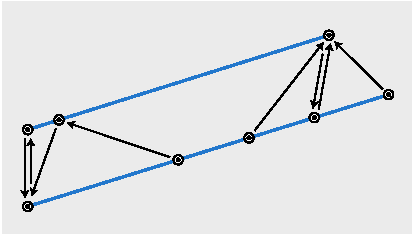
\includegraphics[width=\ScaleIfNeeded]{../chapter4/node-matches}
	\caption{Zuordnung gegenüberliegender \term{nodes} paralleler Linienzüge}
	\label{fig:node-matches}
}



\subsection{Parallelen zusammenfassen}
\label{ch:generalisation-algorithm}

Anhand der Punktezuordnungen können die parallelen Segmente nun zusammengefasst werden.
Hierzu wird ein zufällig ausgewähltes Segment als Beginn eines Linienzugs betrachtet.
Während diesem Linienzug von Segment zu Segment gefolgt wird, können leicht die Mittelpunkte der Punktezuordnungen als Stützpunkte der Mittellinie zwischen den Parallelen verwendet werden (Abbildung~\ref{fig:collapsing-continuation}).

\begin{algorithmhere}{Zusammenfassen}
\label{alg:Zusammenfassen}
\begin{algorithmic}
\State $\textbf{Relation}\ \relation{zusammengefasst} : \textrm{Segment} \rightarrow \textrm{boolean}$
\State $\textbf{Anfangswert}\ \relation{zusammengefasst}[s] \eqdefrel$ nein $\forall\ s$
\Function{Zusammenfassen}{$S, \mathcal{Z}$}\Comment{Segmente $S$, Punktezuordnungen $\mathcal{Z}$}
	\State $E \gets \TheEmptySet$\Comment{Generalisierungsergebnis $E$}
	\ForAll{$s \textbf{ mit } s \in S \wedge \neg\, \relation{zusammengefasst}[s]$}
		\ForAll{$Z \textbf{ mit } Z \in \mathcal{Z} \wedge \textproc{Start}(s) \in Z$}
			\State $t \gets$ mit dem jeweils anderem \term{node} von $Z$ verknüpftes Segment, \\\qquad\qquad\qquad\quad$\hookrightarrow$ welches auf der gleichen Seite von $Z$ liegt wie $s$
			\Repeat
				\Comment{versuchen, die nächste Punktzuordnung $Z'$ zu finden}
				\State $s' \gets \textproc{Fortsetzung}(s,Z,S)$
				\State $\mathtowidth[s']{t'} \gets \textproc{Fortsetzung}(\mathtowidth[s]{t},Z,S)$
				\State $Z_1' \gets \Set{\textproc{Nodes}(s') \cap Z, \textproc{Nodes}(\mathtowidth[s']{t'}) \setminus Z}$
				\State $Z_2' \gets \Set{\textproc{Nodes}(\mathtowidth[s']{t'}) \cap Z, \textproc{Nodes}(s') \setminus Z}$
				\State $Z_3' \gets Z_1' \cup Z_2' \setminus Z $
				\If{$\exists\ Z' : \Set{Z'} = \Set{Z_1', Z_2', Z_3'} \cap \mathcal{Z}$}
					\Comment{Mittellinie bilden}
					\State $E \gets E \cup \Set{(\textproc{Mittelpunkt}(Z), \textproc{Mittelpunkt}(Z'))}$
					\State $\relation{zusammengefasst}[s] \gets$ ja
					\State $\relation{zusammengefasst}[\mathtowidth[s]{t}] \gets$ ja
					\State $s \gets s'$, $t \gets t'$, $Z \gets Z'$ \Comment{weiterschalten}
				\EndIf
			\Until{$\nexists\ Z'$}
		\EndFor
	\EndFor
	\State \textbf{Ergebnis} $E \cup \Set{u \in S \SetCond \neg\, \relation{zusammengefasst}[u]}$
\EndFunction
\end{algorithmic}
\end{algorithmhere}

\onefigure{htb}{
	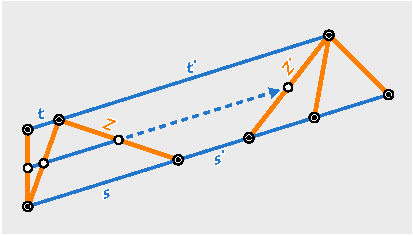
\includegraphics[width=\ScaleIfNeeded]{../chapter4/collapsing-continuation}
	\caption{Bilden der Mittellinie als Generalisierungsergebnis auf Basis der Punkte\-zuordnungen}
	\label{fig:collapsing-continuation}
}

Dabei lässt sich dasjenige Segment, welches jeweils als \textproc{Fortsetzung} eines Linienzugs verwendet wird, wie folgt ermitteln: \nopagebreak

\begin{algorithmhere}{Fortsetzung}
\label{alg:Fortsetzung}
\begin{algorithmic}
\Function{Fortsetzung}{$s, Z, S$}\Comment{Segment $s$, Punktezuordnung $Z$}
	\State $S' \gets \Set{s' \in S \SetCond s' \neq s \wedge \textproc{Nodes}(s) \cap Z \subset \textproc{Nodes}(s')}$
	\State \textbf{Ergebnis} $\begin{cases}s' \in S' & \text{für } |S'| = 1\\\Nil & \text{sonst}\end{cases}$\Comment{nur eindeutige Fortsetzungen}
\EndFunction
\end{algorithmic}
\end{algorithmhere}

Zur Fortführung der Mittellinie werden jeweils drei mögliche Paare von Punkten betrachtet ($Z_1'$, $Z_2'$ und $Z_3'$ in Abbildung~\ref{fig:collapsing-nextmatch}). Nur dann, wenn genau eines von ihnen gleichzeitig einer nach der \textproc{Analyse} identifizierten Punktezuordnung entspricht, wird diese zur Fortführung der Mittellinie verwendet.

\onefigure{htb}{
	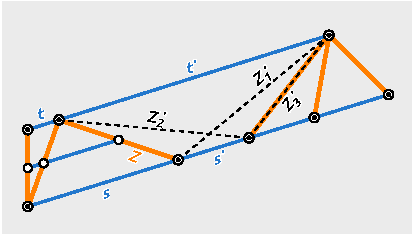
\includegraphics[width=\ScaleIfNeeded]{../chapter4/collapsing-nextmatch}
	\caption
		[Auffinden der nächsten Punktezuordnung zur Fortführung der Mittellinie]
		{Auffinden der nächsten Punktezuordnung zur Fortführung der Mittellinie (im~Beispiel~$Z_3'$)}
	\label{fig:collapsing-nextmatch}
}

Die obenstehende Definition des Algorithmus zum \textproc{Zusammenfassen} ist insofern vereinfacht, als dass sie nicht zur Bildung eines durchgehenden Linienzugs führt, sondern lediglich alle Segmente der Mittellinie sammelt.
Dies kann unschwer bei der Implementierung in Software entsprechend berücksichtigt und angepasst werden.

Ebenso berücksichtigt die Definition weder Kreuzungen noch den Übergang eines einzelnen Linienzugs in zwei parallele Linienzüge.
In diesen Fällen wird die Generalisierung unterbrochen.

Auch der Fall von mehr als zwei Parallelen bleibt der Verständlichkeit der Definition zuliebe unberücksichtigt.
Dies muss bei der Implementierung bedacht werden, da der Begriff „als zusammengefasst markiert“ sonst nicht eindeutig ist.
Der hier beschriebene Algorithmus fasst $n$ parallele Linienzüge zu $n-1$ parallelen Linienzügen zusammen, die jeweils mittig zwischen zwei Parallelen in den Ausgangsdaten liegen.
Eine Erweiterung zur Zusammenfassung einer beliebigen Anzahl von Parallelen auf genau einen Linienzug ist über die Punktezuordnungen möglich, was jedoch in dieser Arbeit nicht weiter betrachtet wird.

% Weiterschaltung ist notwendig, weil ansonsten Endpunkte der generalisierten Linie nicht unbedingt aneinander anstoßen (durch Bildung von "Dreiecken" im Zuordnungsgraphen überlappen sich die Mittellinien u. U.)



\section{Gesamtüberblick}
\label{ch:algorithm-overview}

Setzt man die beschriebenen Algorithmen wie vorgesehen zusammen, so ergibt sich: \nopagebreak

\begin{algorithmhere}{Generalisierung}
\label{alg:Generalisierung}
\begin{algorithmic}
\Function{Generalisierung}{$W$}
	\State $S \gets \textproc{Segmente}(W)$
	\State $S' \gets \textproc{Splitten}(S)$\Comment{Abschnitt~\ref{ch:split-algorithm}}
	\State $\textproc{Analyse}(S')$\Comment{Abschnitt~\ref{ch:analyse-algorithm}}
	\State $\mathcal{Z} \gets \textproc{NodesZuordnen}(S)$\Comment{Abschnitt~\ref{ch:node-match-algorithm}}
	\State $E \gets \textproc{Zusammenfassen}(S, \mathcal{Z})$\Comment{Abschnitt~\ref{ch:generalisation-algorithm}}
	\State \textbf{Ergebnis} $E$
\EndFunction
\end{algorithmic}
\end{algorithmhere}

%Das Ergebnis der Analyse sind Relationen der Segmente untereinander („Segment 1 ist parallel zu Segment 2“).
%Deshalb ist dieser Algorithmus hier ohne Rückgabemenge dargestellt.

Je nach Anwendungsfall sind Nachbearbeitungen und weitere Generalisierungsvorgänge sinnvoll.
In Frage kommen insbesondere die Verknüpfung von aneinander anschließenden Linienzügen sowie eine Formvereinfachung.
Entsprechend der Aufgabenstellung wird darauf hier nicht weiter eingegangen.

Der Rechenaufwand der gesamten \textproc{Generalisierung} lässt sich nicht exakt angeben, da er von der Geometrie der Eingangsdaten abhängt.
So findet das \textproc{Splitten} nur dann statt, wenn \textproc{NaheSegmente} passende \textproc{Fußpunkt}e haben, an denen sie aufgeteilt werden können.
Eine grobe Abschätzung des Rechenaufwands ist jedoch möglich:

In erster Näherung kann davon ausgegangen werden, dass für jeden Punkt genau ein \textproc{Fußpunkt} auf einem anderen (möglicherweise parallelen) Segment gefunden wird, an dem dieses jeweils geteilt wird, dass weitere \textproc{Fußpunkt}e jedoch nicht gefunden werden.
Die Größe der Menge von Segmenten würde damit durch das \textproc{Splitten} verdoppelt:
\[
|S'| \approx 2 \cdot |S|
\]

Tatsächlich werden für \term{real world}--Daten viele \textproc{Fußpunkt}e, an denen Segmente aufgeteilt werden, bei erneuter Lotfällung zum Auffinden weiterer \textproc{Fußpunkt}e und damit zu zusätzlichen Teilungen führen, insbesondere innerstädtisch und in der Nähe von Straßenkreuzungen.
Jedoch werden gleichzeitig auch viele Punkte gar keine \textproc{Fußpunkt}e haben und somit auch nicht zu Teilungen führen, insbesondere in ländlichen Gebieten, wo es insgesamt weniger Straßen und seltener Richtungsfahrbahnen gibt.
Da ländliche Gebiete insgesamt in der Fläche überwiegen, kann angenommen werden, dass $|S'|$ jedenfalls im durchschnittlichen Fall nicht wesentlich größer als $2 \cdot |S|$ ist.

Diese Überlegung bestätigt sich anhand der Betrachtung einer einfachen Autobahn mit zwei Richtungsfahrbahnen:
Hierbei liegen in den Eingangsdaten oftmals Stützpunkte einander gegenüber.
In diesen Fällen werden meist keine \textproc{Fußpunkt}e auf der Gegenfahrbahn gefunden, weil deren Definition eine Mindestlänge~$\mu$ für geteilte Segmente fordert.
Demnach wäre hier $2 \cdot |S|$ als obere Schranke für $|S'|$ im durchschnittlichen Fall zutreffend.

Es seien nun $n \eqdef |S|$ die Anzahl der Segmente in den Eingangsdaten, $\nu$ die durchschnittliche Anzahl der jeweils „nahen“ Segmente und $\psi$ die durchschnittliche Anzahl der Punktezuordnungen je Punkt.
Für die Abschätzung des gesamten Rechenaufwands ergibt sich mit Zählung der geschachtelten Iterationen: \cf{wp:Landau}
\begin{align*}
\textproc{Splitten} &\in \mathcal{O}(2 n \cdot 2 \cdot \nu) = \mathcal{O}(n \cdot \nu)
\\
\textproc{Analyse} &\in \mathcal{O}(2 n \cdot 2 \nu^2) = \mathcal{O}(n \cdot \nu^2)
\\
\textproc{NodesZuordnen} &\in \mathcal{O}(n \cdot 2 \cdot 2) = \mathcal{O}(n)
\\
\textproc{Zusammenfassen} &\in \mathcal{O}(n \cdot \psi)
\end{align*}

Jedoch sind $\nu$ und $\psi$ im Verhältnis zu $n$ vernachlässigbar, weil sie regelmäßig sehr klein sind.
So werden durch die Beschränkung der \textproc{Hülle} auf die unmittelbare Umgebung des jeweiligen Segments nur wenige Segmente als „nah“ betrachtet;
es ist abhängig von der Struktur der Eingangsdaten eine Zahl im unteren zweistelligen Bereich zu erwarten.
%eine nahezu konstante Zahl höchstens im unteren
Weiterhin sind mehr als zwei Punktezuordnungen im Wesentlichen nur im (seltenen) Fall von mehr als zwei erkannten Paralellen zu erwarten.
Mit
\[
\{\nu, \psi\} \subset \hbox{o}(n)
\]
zeigen somit im durchschnittlichen Fall alle Teile der Generalisierung und folglich auch die Generalisierung insgesamt ein lineares Wachstum des Rechenaufwands:
\[
\textproc{Generalisierung} \in \mathcal{O}(n)
\]

%Es ist zu bemerken, dass der Zeitaufwand implementierungsabhängig schneller oder langsamer wachsen kann als der Rechenaufwand.

Im \emph{schlechtesten} Fall liegen alle Segmente so nah beieinander und haben so ungünstige Winkel, dass \emph{alle} Segmente solange aufgeteilt werden, bis \emph{jede} weitere Teilung zur Unterschreitung der Mindestlänge~$\mu$ führen muss.
An diesem Punkt bricht das \textproc{Splitten} ab, weil die Einhaltung der Mindestlänge definitionsgemäß Bedingung für die Existenz eines \textproc{Fußpunkt}s ist.
Die Größe der Menge $S'$ und damit der weitere Rechenaufwand hängen dann von der geometrischen Länge der Segmente und der Wahl von $\mu$ ab.
Eine solche Situation ist allerdings in \term{real world}--Daten für ein Straßennetz wenig wahrscheinlich.
Sie könnte nur dann überhaupt auftreten, wenn der Höchstabstand $\eta$ für \textproc{NaheSegmente} zu groß gewählt wurde (vgl. Abschnitt~\ref{ch:split-algorithm}).

Selbst in diesem schlechtesten Fall terminieren die Algorithmen.
Für das \textproc{Splitten} wurde dies soeben begründet; für alle anderen imperativ beschriebenen Algorithmen ist es trivial zu erkennen, da sie nur über endliche unveränderliche Mengen iterieren.
% - terminierend: ja, weil alle Schleifen auf abschließenden Mengen arbeiten, mit Ausnahme des Splittens, wobei aber durch die minimale Fragmentlänge µ eine klare Abbruchbedingung gegeben ist

Die Algorithmen arbeiten jedoch nicht deterministisch:
Abhängig von den Eingabedaten ist anzunehmen, dass je nach Reihenfolge der Iteration das \textproc{Splitten} und damit auch die \textproc{Analyse} unterschiedliche Ergebnisse liefern.
Es ist jedoch nicht zu erwarten, dass diese Varianzen großen Einfluss auf das Ergebnis haben.
% - deterministisch: nein; erstens abhängig von Input denkbar, dass je nach Reihenfolge der Iteration das Splitten und damit die Analyse unterschiedliche Ergebnisse liefert; zweitens Länge der generalisierten Linienzüge zufallsabhängig (da "rückwärts" nicht spezifiziert); jedoch nicht zu erwarten, dass diese Varianzen großen Einfluss auf das Ergebnis haben

Auf eine formale Festlegung der Kriterien für die Korrektheit der Generalisierung wurde verzichtet.
% "korrekt": nicht definiert, also nicht nachweisbar; Nachweis würde auch den Rahmen sprengen
Um nachzuweisen, dass die entwickelten Algorithmen funktionieren, wurden diese stattdessen ausführbar in Software implementiert.
Dies beschreibt Kapitel~\ref{ch:impl}.
Im Anschluss daran werden in Kapitel~\ref{ch:result} das Generalisierungsergebnis und die Praxistauglichkeit der Algorithmen für unterschiedliche Fälle diskutiert.



% single-chapter commands
%\onlyinsubfile{\listoffigures}
%\onlyinsubfile{\subfile{../bibliography/Literaturverzeichnis}}
\end{document}
